\section{Background}

Our team includes members who bring a variety of complementary
technical strengths to address the opportunity presented by our
insight that prescriptions are programs. Belknap led a team who
implemented the first patient-oriented prescription, \emph{on
  paper}. Findler and Flatt built and maintain Racket, a platform for
building domain-specific languages. The next two subsections explain
our experience in more detail.

\subsection{Prescriptions as Programs}\label{sec:pap}

Physicians usually rely on memory and write extemporaneous
prescriptions. Occasionally, physicians use standard order sets or
templates~\citep{Elsberry1978,Honda1979,Kowalsky1982}, but these are
rarely derived explicitly from scientific
evidence~\citep{Fonarow2007,Dranitsaris2001}, often violate principles
of good software design, and are not verifiably debugged. Standard
order sets or templates have been shown to improve compliance with
drug therapy recommendations in some settings \citep{Girotti1990} but not in
others \citep{Aswapokee1992}. Prescription bugs in standard order sets can cause
catastrophic medication errors \citep{Cohen1992}.

The apparent simplicity of prescriptions is deceptive, as the
prescriber's terse instructions rely implicitly on subroutines:
toxicity and efficacy monitoring, pharmaceutical compounding, pharmacy
and nursing practices, operating instructions, laboratory methods, and
standard operating procedures. Neglect of scientific evidence, poor
design, and lack of adequate debugging of prescriptions and their
subroutines likely account for their erratic and occasionally fatal
effects. The recognition of the algorithmic nature of prescriptions
compels the application of software design principles and debugging
methods to their improvement.

The medical community has acknowledged that there has been no method
to ensure the rapid, reliable translation of detailed knowledge about
drug safety, efficacy, and cost into clinical practice. Clinical
practice guidelines have been variously criticized as being vague,
untested, non-rigorous~\citep{Weingarten1997},
obsolescent~\citep{Shekelle2001} and are largely ignored by
physicians~\citep{Cabana1999}. A recent, seminal study has found that
there has been little or no progress in improving the safety of
patients over the past ten years, despite advances in understanding
and mitigating some types of medical error~\citep{Landrigan2010}.

While it is possible for a physician to order drug therapy without
consulting relevant research articles, clinical practice guidelines,
expert opinions, textbooks, or lectures, a physician cannot order drug
therapy without a prescription. That is, the prescription is located
on the critical path between intent and practice. Well-formed, widely
used prescriptions exert beneficial effects through reduction of
clinical process variation, familiarity to clinicians, and
displacement of unsafe or ineffective practices. When properly
designed and debugged, prescriptions provide a conduit through which
evidence-based medical knowledge can reliably and safely reach patients.

We applied this insight to significantly reduce the risk of severe injury from medical use of opiods among hospitalized adults at St.\ Francis Medical
Center in Peoria, IL, a 731-bed tertiary care academic medical
center~\citep{Belknap2008}. During a 1 year base-line period, there were three to seven severe or fatal opioid-associated adverse drug events (ADEs) each month. After widespread adoption of POPA, the rate of severe/fatal opioid ADEs dropped to zero/month. Figure~\ref{fig:popa} shows POPA, the
complete program that we developed as part of our study.

Clinicians who use these patient-oriented prescriptions provide assiduous peer review, compelling the translation of new medical knowledge into improved
prescriptions. Sound prescription design followed by iterative cycles of hazard identification and debugging reduces the rate of severe patient injury by eliminating the prescription bugs that are a root cause of opioid-associated ADEs. POPA was subsequently implemented in two other hospitals. As POPA does not depend on resources that are unique to our hospital, we
expect that POPA is widely applicable.

Consider the subroutine for fentanyl dose reduction:
\begin{center}
\fbox{\scriptsize\begin{tabular}{ll}
\textit{Taper:} & 
\parbox[t]{5.2in}{STOP on-demand dose after (3 days) \underline{\hbox
  to 1in{}} (Alternatively, enter a stop date) \& \textit{then} REDUCE
continuous dose rate every 5 hours by (10) \underline{\hbox to .4in{}}
micrograms}\\
\end{tabular}}
\end{center}

\noindent
This fragment represents a subroutine that is executed by humans. This
human-oriented programming language 
includes conditionals, an optionally specified
variable with default value, an external (human) processor call, and
elements driving reconciliation with other subroutines. The phrasing
also employs TALLMAN lettering to emphasize the direction of
change. The content of this prescription is
evidence-based. Its structure was based on software design principles
and then debugged, through trial and error, deriving a form that is
clear to clinicians and accurate in performance. For example, 
constructions like TALLMAN lettering improved execution accuracy compared with
less redundant code. Unlike CPOE data tables
that obscure the hierarchical and modular structure of prescriptions,
this fragment of a \poppl{} program clarifies it, opening the door to 
the use of computer science techniques for improving the quality of
the program.

\begin{figure}
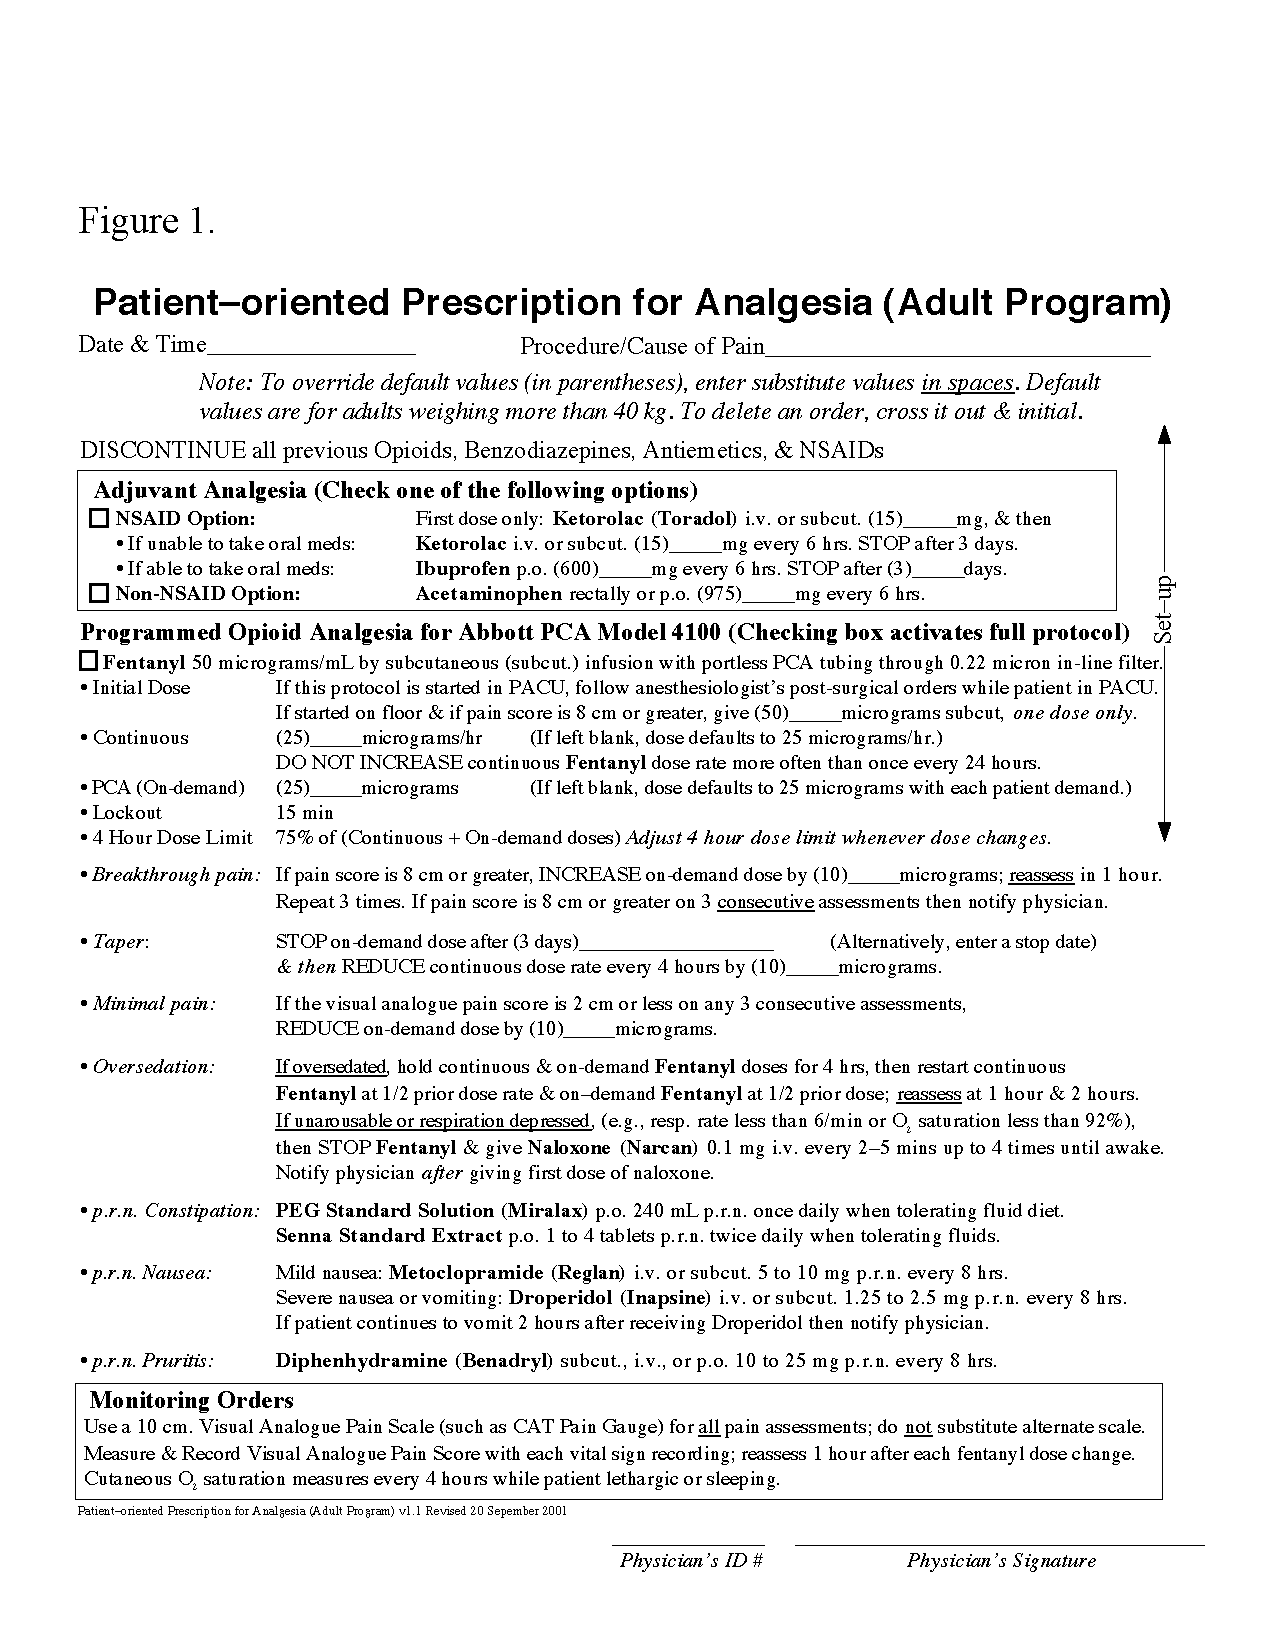
\includegraphics[scale=.8]{fig1.pdf}
\captionsetup{labelformat=empty}
\caption{}\label{fig:popa}
\end{figure}

 
To validate the success of our original \poppl{} program, we also
conducted a statistical process control clinical trial and nested
subcohort analysis in a population of 153,260 hospitalized adults. In
the orthopedics subcohort, POPA increased recording of pain scores
(94\% vs.\ 72\%, P $<$ 0.00001) and use of adjuvant analgesics (95\%
vs.\ 40\%, P $<$ 0.00001) and resulted in fewer opioid-associated
severe adverse drug events than routine patient-controlled analgesia
(PCA) (0\% vs.\ 2.7\%, number needed to treat (NNT) = 35, P $<$
0.015). Hospital-wide, POPA use increased to 62\% of opioid
prescriptions (diffusion half-life = 98 days), while opioid-associated
severe/fatal adverse drug events fell from an initial peak of seven
per month to zero per month during the final 6 months (P $<$ 0.0016)
of the study, as shown in Figure~\ref{fig:popa-results}.

\begin{figure}
\begin{center}
\includegraphics[scale=.2]{popa.png}
\end{center}
\caption{POPA Trial results}\label{fig:popa-results}
\end{figure}

The success of the POPA was due in part to the rigor that algorithmic
thinking brought to the process of building the prescription and in
part to extensive debugging. This proposal aims to build, test, and
deploy the software required to make \poppl{} programs
machine-executable, interoperable with other healthcare software, and
available for clinical trials in routine clinical environments.

\subsection{Specialized Programming Languages in Racket}\label{sec:racket}

The Racket programming language~\citep{Racket} offers an extensible
core language, and the DrRacket programming
environment~\citep{DrSchemeJFP} is (by design) adaptable to language
extensions. The environment part of the equation is crucial, because
domain experts need more than a compiler and run-time system to
develop programs. They also need a full suite of development tools,
including program editors, interactive evaluators, debuggers,
syntax-coloring editors, and documentation tools. Prescribers write
complex medical algorithms and are familiar with algorithmic thinking
but very few have any formal knowledge of programming. Thus, a key
design element for POP-PL will be usability by prescribers with little
formal knowledge of computer programming. There are numerous instances
where such software has been constructed in other domains; consider,
for example, that administrative assistants use Excel and machine
operator at Caterpillar Tractor program lathes. These are domain
specific languages that allow people to program with little formal
training. Doctors are programmers too; they write prescriptions and use
order sets~\cite{Elsberry1978,Honda1979,Kowalsky1982}. These are
rarely derived from evidence~\cite{Dranitsaris2001,Fonarow2007}, often
violate software design principles, and are not verifiably
debugged. Standard order sets increase use of best practices in some
settings~\cite{Girotti1990} but not others~\cite{Aswapokee1992}. Bugs in order
sets can cause catastrophic errors~\cite{Cohen1992}.

VisiCalc, the first spreadsheet app, resembled paper accounting
worksheets but revolutionized accounting and finance because it did
something radically different, auto–calculating data cell values
according to formulas programmed by the user. Previously, this work
required calculators, pencils, and paper, and was laborious and
error-prone. Our task here is similar; the design and implementation
of POP-PL, a prescribing language, will be a process of discovery, as
we study the (often elegant) prescriptions clinicians already use. We
expect to develop a language that will leverage the existing
knowledge, tropes, and structures that physicians and other
prescribers have. We envision an ``active prescription'' that
superficially resembles a paper prescription in the same way that the
GUI of Excel resembles a paper spreadsheet.

DrRacket is best known in its role as a tool for
teaching; the teaching dialect of Racket is not the full language, but a series of
languages designed for progressively more advanced
students---domain-specific languages for introductory programming.
Other domain-specific languages that are embedded in
Racket include the Redex language for developing and testing
operational semantics~\citep{Redex}, the web-server framework for
transparently implementing web services via sessions managed over
HTTP~\citep{web-server,mccarthy09,mccarthy10}, the Slideshow language
for creating slide presentations~\citep{Slideshow}, the Scribble
language for documentation and typesetting other forms of prose~\citep{Scribble}, and
the Margave tool for security policy verification~\citep{Margave}.

Of these, Margave most closely resembles the use of Racket  we have in mind
for prescription programs. Experts in the domain of security protocols
use Margave as a language within DrRacket, but do not write
Racket code at all. Instead, they treat DrRacket as a kind of
``DrMargave,'' since writing a module in the Margave language causes 
DrRacket to adapt to that specific domain language.

Racket's underlying language-definition technology is based on
Lisp-style macros---specifically, the lexical-context preserving macro technology that evolved in
Scheme~\citep{R6RS}. Racket builds on this foundation with a 
richer API for macro transformers to manipulate and inspect syntactic
terms. This API is powerful enough, for example, to implement the
continuation-passing transformation of the web-server
framework~\citep{mccarthy09}, the type checker for a
statically typed dialect of Racket~\citep{TypedRacket}, as well as the
Racket class system itself \citep{fff:scheme-classes-mixins-traits}. Macros are
integrated into a module layer that enables different languages and
language extensions to compose within a larger program.
